\subsection{Services}

\begin{frame}
  \frametitle{Services}
  \begin{itemize}
  \item Services are components running in the background
  \item They are used either to perform long running operations or
    to work for remote processes
  \item A service has no user interface, as it is supposed to run when the
    user does something else
  \item From another component, you can either work with a service in
    a synchronous way, by \emph{binding} to it, or asynchronous, by
    \emph{starting} it
  \end{itemize}
\end{frame}

\begin{frame}[fragile]
  \frametitle{Service Manifest}
\begin{minted}{xml}
<?xml version="1.0" encoding="utf-8"?>
<manifest package="com.example.android">
    <application>
        <service android:name=".ExampleService"/>
    </application>
</manifest>
\end{minted}
\end{frame}

\begin{frame}
  \frametitle{Services Types}
  \begin{itemize}
  \item We can see services as a set including:
    \begin{itemize}
    \item Started Services, that are created when other components
      call \code{startService}. Such a service runs as long as needed,
      whether the calling component is still alive or not, and
      can stop itself or be stopped. When the service is stopped, it
      is destroyed by the system
      \begin{itemize}
      \item You can also subclass \code{IntentService} to have a
        started service. However, while much easier to implement, this
        service will not handle multiple requests simultaneously.
      \end{itemize}
    \item Bound Services, that are bound to by other components by
      calling \code{bindService}. They offer a client/server like
      interface, interacting with each other. Multiple components can
      bind to it, and a service is destroyed only when no more
      components are bound to it
    \end{itemize}
  \item Services can be of both types, given that callbacks for these two do
    not overlap completely
  \item Services are started by passing Intents either to the
    \code{startService} or \code{bindService} commands
  \end{itemize}
\end{frame}

\begin{frame}
  \frametitle{Services Lifecycle}
  \begin{figure}[h!]
    \centering
    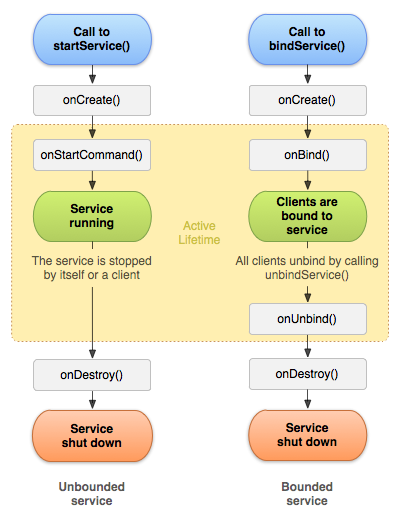
\includegraphics[height=0.8\textheight]{slides/android-application-services/service-lifecycle.png}\\
    {
      \tiny
      Credits: \url{http://developer.android.com}
    }
  \end{figure}
\end{frame}

\begin{frame}
  \frametitle{Bound Services}
  \begin{itemize}
  \item There are three possible ways to implement a bound service:
    \begin{itemize}
    \item By extending the \code{Binder} class. It works only when the
      clients are local and run in the same process though.
    \item By using a \code{Messenger}, that will provide the interface
      for your service to remote processes. However, it does not
      perform multi-threading, all requests are queued up.
    \item By writing your own AIDL file. You will then be able to
      implement your own interface and write thread-safe code, as you
      are very likely to receive multiple requests at once
    \end{itemize}
  \end{itemize}
\end{frame}

\begin{frame}
  \frametitle{Bound Services and Started Lifecycle}
  \begin{figure}[h!]
    \centering
    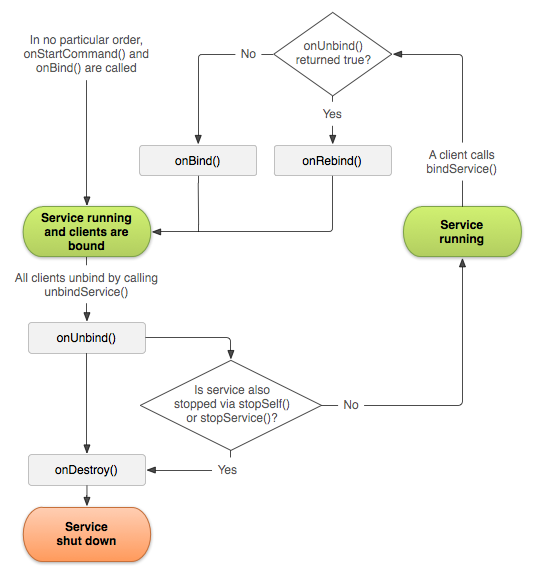
\includegraphics[height=0.8\textheight]{slides/android-application-services/service-start-bound-lifecycle.png}\\
    {
      \tiny
      Credits: \url{http://developer.android.com}
    }
  \end{figure}
\end{frame}
